%!TEX program = lualatex
%% LyX 2.0.0 created this file.  For more info, see http://www.lyx.org/.
%% Do not edit unless you really know what you are doing.
\documentclass[12pt,a4paper,english,british]{article}
\usepackage[T1]{fontenc}
\usepackage[utf8]{luainputenc}
\usepackage{listings}
\usepackage{verbatim}
\usepackage{varioref}
\usepackage{refstyle}
\usepackage{textcomp}
\usepackage{amstext}
\usepackage{graphicx}
\usepackage{babel}
\usepackage[margin=2cm]{geometry}
\renewcommand{\baselinestretch}{1.5}

\makeatletter

%%%%%%%%%%%%%%%%%%%%%%%%%%%%%% LyX specific LaTeX commands.

\AtBeginDocument{\providecommand\subref[1]{\ref{sub:#1}}}
\DeclareRobustCommand{\greektext}{%
  \fontencoding{LGR}\selectfont\def\encodingdefault{LGR}}
\DeclareRobustCommand{\textgreek}[1]{\leavevmode{\greektext #1}}
\DeclareFontEncoding{LGR}{}{}
\DeclareTextSymbol{\~}{LGR}{126}
%% Because html converters don't know tabularnewline
\providecommand{\tabularnewline}{\\}
\RS@ifundefined{subref}
  {\def\RSsubtxt{section~}\newref{sub}{name = \RSsubtxt}}
  {}
\RS@ifundefined{thmref}
  {\def\RSthmtxt{theorem~}\newref{thm}{name = \RSthmtxt}}
  {}
\RS@ifundefined{lemref}
  {\def\RSlemtxt{lemma~}\newref{lem}{name = \RSlemtxt}}
  {}

%%%%%%%%%%%%%%%%%%%%%%%%%%%%% END LyX specific LaTeX commands.

\makeatother


\begin{document}
\pagebreak{}


\title{Runtime Array Fusion\\
for Data Parallelism\\
\ \\
Masters Thesis [Draft]}


\author{Georgy Roldugin}

\maketitle
~\\
\\


\begin{center}

\includegraphics{img/UNSW_PortraitGreyscale_Black}
\par\end{center}

~\\
\\


\begin{center}

\par\end{center}

\begin{center}
\begin{tabular}{ll}
\textbf{Supervisor} & Manuel Chakravarty~~~~~\tabularnewline
\textbf{Co-Supervisor} & Gabriele Keller\tabularnewline
\textbf{External Supervisor} & Ricardo Peña\tabularnewline
\end{tabular}
\par\end{center}

\thispagestyle{empty}

\pagebreak{}


\section{Introduction}

\begin{comment}
The need for the research (aims, problem statement and justification)
½ to 1page introduction
\end{comment}


The past decade has seen a rise in development of increasingly sophisticated
multi-core and multi-processor computer systems. From the early hyperthreaded
solutions boosting the performance of interleaved IO and CPU bound
computations, to the modern architectures comprising of a number of
independent processing cores, the horsepower for demanding applications
is now available even in the most affordable consumer systems. The
high grade systems targeting scientific applications exposing a large
amount of parallelism combine multiple processors with multiple cores,
where each of the cores can run a number of hardware scheduled threads.

While the hardware for running highly parallel computations is available
and is improving at a high pace, the development of such applications
targeting an arbitrary number of processing elements (be that cores,
processors or hardware threads) is often a challenging task. The problems
involved are finding an appropriate parallel implementation of the
task at hand, implementing it such that the computations are evenly
distributed across processing elements and synchronising parallel
computations when necessary. The latter two require a substantial
programmer's intervention to get the algorithm running fast. %
\begin{comment}
It is not uncommon for the initial parallel implementation to run
only slightly faster than the sequential version.
\end{comment}
{} The resulting application is a mixture of the actual algorithm and
the implementation specific code, dealing with concurrency and parallelism.
This obscures code clarity and may generally be error-prone.

One alternative to this practice of explicit parallelisation is to
provide a common set of operations on large data structures. Programs
implemented in terms of these operations would be automatically parallelised
across the available processing elements. This approach is exercised
by several frameworks covering a number of host languages, target
architectures and suitable applications domains \cite{PLKC08,KCL+10,CKL+11,AS07}.
In the pursuit of a high level view of the problem a major inefficiency
is introduced. Having provided a number of primitive operations the
problem of multiple traversals arises. In a manually written program
the programmer could merge multiple primitive operations into one.
That would only traverse a data structure once keeping the memory
traffic to the necessary minimum and utilising cache correctly. On
the other hand a straight forward high level library implementation
would potentially traverse the same data structure in each operation.
For large data structures this may lead to poor cache utilisation
and high memory traffic. Additionally the operations may allocate
temporary data structures to store their intermediate results which
leads to further memory and runtime penalties. Optimising out the
superfluous data structure traversals and allocations is collectively
referred to as Loop Fusion. It allows to transform a program expressed
in terms of high level operations into a program that would be semantically
comparable to a handwritten one. The following chapters provide the
motivation behind fusion, introduce the context of the project as
well as the previous work in the field. A research proposal and a
planned list of milestones are provided in the final chapters.

\pagebreak{}


\section{Motivation}

Suppose we have the following computation to perform:

\begin{lstlisting}[basicstyle={\ttfamily},language=Haskell,tabsize=4]
sum (zipWith (*) xs ys)
\end{lstlisting}


A person familiar with the fundamentals of functional programming
is likely to spot the computation of the dot product of two vectors
in this snippet of Haskell code. Indeed, the $zipWith$ list combinator
conventionally creates a list, whose elements are calculated by applying
some given function to the elements of the input lists occurring at
the same positions in both lists. In the above case {}``zipping''
with the product as the function will element-wise multiply the two
vectors $xs$ and $ys$. Quite expectedly the $sum$ combinator will
sum the elements of the resulting vector into a scalar value, yielding
the dot product of $xs$ and $ys$.

This one-liner was an attempt to develop the motivation for the high-level
view on numeric computations. It may seem reasonable to replace the
lists with arrays and reimplement the same high-level interface in
terms of traditional arrays to avoid random memory access penalties
as in the case of lists. Providing an instantly familiar interface
without compromising performance has been one of the goals of the
Data Parallel Haskell (DPH) project \cite{PLKC08,CLP+07}. The work
in this thesis has been carried out in the context of this project.
It will be discussed in more detail in section \ref{sec:Lit:DPH}.

However, even if we replaced the lists with arrays and gave efficient
implementations to $sum$ and $zipWith$, the resulting algorithm
is still likely to be slower than on written by hand. The $zipWith$
combinator produces an intermediate array containing the element-wise
product of the two input vectors. It is immediately consumed by $sum$,
yielding the final (scalar) value. Thus the algorithm performs two
traversals and allocates another array of the size of the input arrays.
The same algorithm could be expressed by the following function in
C:

\begin{lstlisting}[basicstyle={\ttfamily},language=C,tabsize=4]
double dotProduct (int len, double xs[], double ys[]) {
	int i;

	double* temp = malloc(sizeof(double)*len);
	for(i=0; i<len; ++i)
		temp[i] = xs[i]*ys[i];

	double result = 0;
	for(i=0; i<len; ++i)
		result += temp[i];

	return result;
}
\end{lstlisting}


It should be obvious that the same result could be achieved by using
a single loop computing the final result incrementally without allocating
a temporary array as in the following:

\begin{lstlisting}[basicstyle={\ttfamily},language=C,tabsize=4]
double dotProduct (int len, int[] xs, int[] ys) {
	double result = 0;
	int i;
	for(i=0; i<len; ++i)
		result += xs[i]*ys[i];
	return result;
}
\end{lstlisting}


The process of finding and exploiting the opportunities for squashing
multiple loops into one is referred to as loop fusion. Another term
for this commonly encountered in literature is deforestation, first
coined by Philip Wadler in \cite{Wad90}. In reality the code in the
the above examples has been optimised in two ways. Just fusing the
two loops together on the basis that they iterate over the same range
would have produced:

\begin{lstlisting}[basicstyle={\ttfamily},language=C,tabsize=4]
for(i=0; i<len; ++i) {
	temp[i] = xs[i]*ys[i];
	result += temp[i];
}
\end{lstlisting}


which does not completely bypass the extra allocation. The optimisation
that gets rid of the unnecessary temporary arrays and is commonly
applied when fusing loops, is called scalarisation or, more generally,
array contraction. During this optimisation we attempt to remove a
dimension from the array. In this particular case we contracted a
one dimensional array to a scalar, hence scalarisation. However, in
the examples with arrays of higher dimensions the dimension could
just be reduced, and not eliminated entirely.

The work described in this thesis is oriented towards complementing
the fusion mechanisms%
\footnote{While there is the distinction between loop fusion and array contraction,
in many cases throughout this document the term $fusion$ will be
used to describe both optimisations applied together. %
} currently employed in DPH. In the remainder of this chapter we will
introduce the reader to the Data Parallel Haskell (DPH) project and
similar systems, progressing to the description of some of the most
common fusion systems.

\pagebreak{}


\section{\label{sec:Lit:DPH}Context}

Data Parallel Haskell is an active library for the Haskell programming
language, providing high level access to nested data parallelism.
The above definition may seem complicated at first and should probably
be backed up by a set of explanations:
\begin{itemize}
\item Nested data parallelism is a type of SPMD parallelism, which operates
on irregular data structures. Some of the examples of irregular data
structures are sparse matrices and unbalanced trees
\item An active library may be defined as one which takes active part in
the optimisation and the compilation of its client code. Indeed, DPH
guides the compilation process in many ways including choosing the
data representation \cite{CDL09} and applying rewrite rules \cite{PTH01}
to improve performance. In fact, a major part of DPH -- the vectoriser
-- is implemented in the Glasgow Haskell Compiler%
\footnote{Glasgow Haskell Compiler: http://www.haskell.org/ghc%
} (GHC).
\end{itemize}
In essence, DPH reimplements the familiar list interface in terms
of seamlessly parallelised arrays. Figure \ref{fig:Lit:DPH-interface-functions}
lists some of the most important functions in the DPH interface. Since
DPH has language support, the bracket notation for parallel arrays
closely resembles that for Haskell lists: \lstinline[basicstyle={\ttfamily}]![:a:]!
denotes a parallel array of type \lstinline[basicstyle={\ttfamily}]!a!.
The counterpart of Haskell's list comprehensions is also present and
is called \emph{parallel array comprehensions.}

\begin{figure}
\begin{lstlisting}[basicstyle={\ttfamily},language=Haskell,tabsize=4]
(!:)		:: [:a:] -> Int -> a
sliceP		:: [:a:] -> (Int,Int) -> [:a:]
replicateP	:: Int -> a -> [:a:]
mapP		:: (a->b) -> [:a:] -> [:b:]
zipP		:: [:a:] -> [:b:] -> [:(a,b):]
zipWithP	:: (a->b->c) -> [:a:] -> [:b:] -> [:c:]
filterP		:: (a->Bool) -> [:a:] -> [:a:]

concatP		:: [:[:a:]:] -> [:a:]
concatMapP	:: (a -> [:b:]) -> [:a:] -> [:b:]
unconcatMapP:: [:[:a:]:] -> [:b:] -> [:[:b:]:]
transposeP	:: [:[:a:]:] -> [:[:a:]:]
expandP		:: [:[:a:]:] -> [:b:] -> [:b:]

combineP	:: [:Bool:] -> [:a:] -> [:a:] -> [:a:]
splitP		:: [:Bool:] -> [:a:] -> ([:a:], [:a:])
\end{lstlisting}


\caption{\selectlanguage{english}%
\label{fig:Lit:DPH-interface-functions}\foreignlanguage{british}{Type
signatures for parallel array operations.}\selectlanguage{british}
}
\end{figure}


Collective operations on parallel arrays are executed in parallel
when hardware supports it. Currently, a backend supporting Haskell
threads \cite{Jones08atutorial} exists. Due to the flexible design
of the library, support for other parallel architectures may be added
in the future. By design the computation is split evenly across processing
elements even for highly irregular parallel programs. The remainder
of the section will outline the library structure, cover the basics
of vectorisation and describe the current stages of fusion in DPH.


\subsection{Vectorisation}

The main goal behind DPH was to allow the programmer to write parallel
programs without worrying about scheduling, load balancing and low
level optimisations. The work on DPH was originally inspired by Blelloch's
pioneering work on NESL \cite{BCH+}, a research language designed
specifically to explore the potential of the new approach to nested
data parallelism.

\begin{figure}
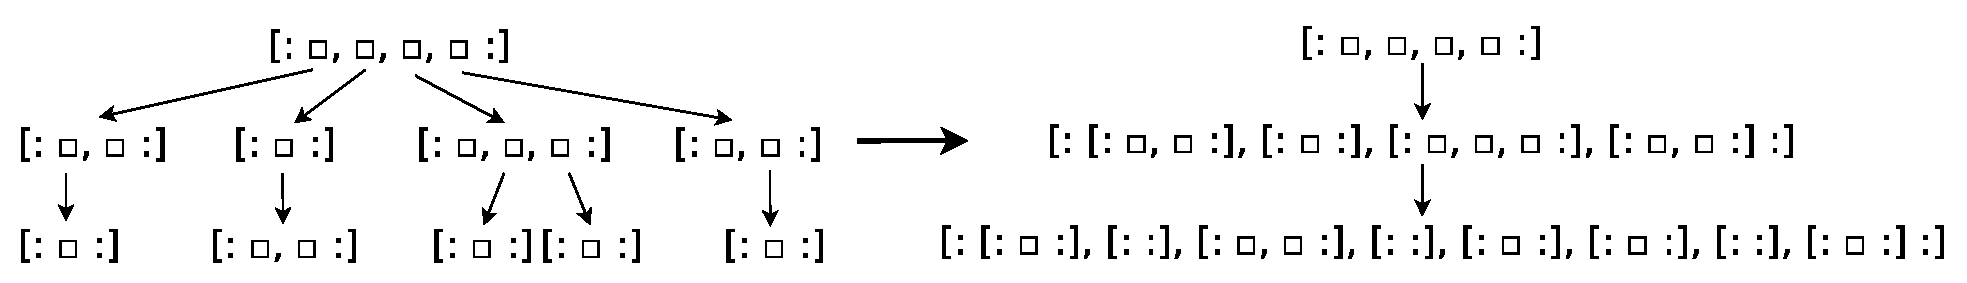
\includegraphics[width=1\textwidth]{img/TreeRepr}

\caption{\selectlanguage{english}%
\label{fig:Lit:Tree}\foreignlanguage{british}{Value of type \texttt{{[}:Tree:{]}}
and its vectorised representation. Empty subtrees are omitted from
the conceptual representation.}\selectlanguage{british}
}
\end{figure}


If we were to take a tree of an arbitrary shape and tried to apply
some computation to its every node in parallel, a naive tree representation
would have probably failed to provide us with enough clues on how
to split the load between processing elements. Suppose we store an
element of type \texttt{Int} and an array of subtrees at each node.
Then the tree can be expressed as

\begin{lstlisting}[basicstyle={\ttfamily},language=Haskell,tabsize=4]
data Tree = Tree Int [:Tree:]
\end{lstlisting}


A sample tree is given in Figure \ref{fig:Lit:Tree}. Just by looking
at the top level of the tree it would not be possible to know the
branching. What vectorisation does is it translates user programs
that use nested data parallelism to those using flat data parallelism.
Figure \ref{fig:Lit:Tree} presents the same tree with each of its
levels placed into a parallel array. At the implementation level it
is flattened even further by storing a flat data array with all the
node values and a \emph{segment descriptor }defining the partitioning
to recreate the original nesting. Thus, a parallel array with elements

\begin{lstlisting}[basicstyle={\ttfamily},language=Haskell]
[: [:5:],[::],[:4,2:],[::],[:3:],[:17:],[::],[:11:] :]
\end{lstlisting}


which may have been the deepest level of the discussed tree, would
have been stored as an array of unboxed values

\begin{lstlisting}[basicstyle={\ttfamily},language=Haskell]
[# 5, 4, 2, 3, 17, 11 #]        -- data
\end{lstlisting}


together with the segment descriptor containing the lengths and the
starting index positions of the contained arrays (offsets into the
data array):

\begin{lstlisting}[basicstyle={\ttfamily},language=Haskell]
([# 1, 0, 2, 0, 1, 1, 0, 1 #],  -- lengths
 [# 0, 1, 1, 3, 3, 4, 5, 5 #])  -- indices
\end{lstlisting}



\subsection{\label{sub:DPH-Data-Repr}Data Representation}

Together with flattening, the vectoriser chooses the best representation
for the data, e.g. for sum types and product types. Haskell's product
types, or the tuples of two of more heterogeneous elements, are allocated
as boxed values on the heap. Storing an array of pointers to heap
allocated values would have been a major hit on performance due to
the costs of unboxing as well as loading the individual values from
memory instead of fetching multiple at a time. Instead, an array of
pairs \texttt{{[}:(a,b):{]}} is stored as a pair of arrays \texttt{({[}:a:{]},{[}:b:{]})}.

Similarly, the sum types, or the user defined ADT's, are stored as
tuples of arrays. Having multiple arrays, each storing the interesting
values wrapped by the same constructor, not only avoids the cost of
unboxing but also facilitates pattern matching on constructors. Thus
the values constructed by the same constructor are stored in the same
array. The penalty paid is keeping a selector array to recreate the
original interleaving. Quite clearly sum types and product types can
be recursively nested.%
\begin{comment}
TODO: give an example of sum types and their representation in parrs
\end{comment}


We have discussed the way the data is represented in DPH but said
nothing about how the vectoriser adapts the functions to fit the new
data representation. We do not need to delve into too much detail
here, since by the time we get to the backend of the library (where
the fusion takes place) we are no longer interested in how it's done.
One important intuition to develop can be illustrated by the following:

\begin{lstlisting}[basicstyle={\ttfamily},language=Haskell]
f :: Float -> Float
f x = x*x + 1
\end{lstlisting}


For every such function the vectoriser generates its \emph{lifted
}version \texttt{f\textasciicircum{}} thus:

\begin{lstlisting}[basicstyle={\ttfamily},language=Haskell]
f^ :: [:Float:] -> [:Float:] -> [:Float:]
f^ x = (x *^ x) +^ (replicateP n 1)
       where n = lengthP x
\end{lstlisting}


This new definition obeys the equation \texttt{f\textasciicircum{}
= mapP f}, thus it is possible to replace \texttt{(mapP f)} with \texttt{f\textasciicircum{}}.
Now if we return to the tree example, there we may need to apply \texttt{f
}to an array of arrays. The flat data representation we chose above
allows us to easily derive \texttt{f\textasciicircum{}\textasciicircum{}}
in terms of \texttt{f\textasciicircum{}} like this:

\begin{lstlisting}[basicstyle={\ttfamily},language=Haskell]
f^^ :: [:[:Float:]:] -> [:[:Float:]:]
f^^ xss = unconcatP xss (f^ (concatP xss))
\end{lstlisting}


Recalling that we use a flat data array together with a segment descriptor
to represent \texttt{xss}, it becomes clear that both \texttt{concatP}
and \texttt{unconcatP} are simple constant time operations that do
nothing more than replacing one segment descriptor with another.

Vectorisation is more thoroughly covered in the tutorial-style paper
\cite{PLKC08}.


\subsection{Backend and Fusion}

By the time the backend is reached the nesting in the original user
program is only defined in terms of segment descriptors where required.
As discussed in the previous section the vectoriser has also stripped
out the product and sum types including those defined by the user
and conveniently arranged them in flat data arrays. Thus, the backend,
or the library of primitive operations, needs only support the arrays
of primitive types. Since some of the operations on nested arrays
need to respect the boundaries of the inner arrays (e.g. reductions),
the segmentation information is still present.

The primitive library implements a fixed interface that is called
by the vectoriser. The support for any architectures other than multi-core
systems can be added through reimplementing the primitive library
interface, though the parallel programming model heavily relies on
shared memory architectures for efficiency. The primitive library
in its current state uses the Vector library%
\footnote{http://hackage.haskell.org/package/vector%
} to store arrays and Haskell threads to implement parallelism \cite{Jones08atutorial}.
Essentially each thread is given a chunk of array(s) and a sequential
operation to apply to it.

\label{Lit:DPH-fusion-levels}DPH introduces fusion at three different
levels:
\begin{enumerate}
\item Removing synchronisation points\\
Due to the use of Haskell threads, the code responsible for distributing
the processing across the processing elements introduces many fork/join
points. Due to the specifics of the other two fusion levels, this
does not allow the fusion to be applied. Thus, if there is no processing
to be done between the join and the next fork, these are fused together
using the rewrite rules \cite{PTH01}. One problem with this approach
is that the rewrite happens unconditionally when matched, which may
lead to unbalanced load, e.g. after a \texttt{filter} operation.
\item A minimal set of sequential rewrite rules\\
Just like removing superfluous synchronisation points, some adjacent
array operations can be optimised away with the help of rewrite rules.
An example of an easy optimisation would be on two consecutive maps
on the same array, i.e. \texttt{map f (map g xs) = map (f . g) xs}.
While these optimisations are quick and effective, it is not feasible
to come up with a rewrite rule for every pair of fusible operations.
A small set of such rewrite rule is employed in DPH to get rid of
the most common combinations at a relatively low cost.
\item Stream Fusion\\
Stream fusion receives the most attention as far as the fusion in
DPH goes. It not only considerably affects the internal implementation
of primitive operations in DPH and in the Vector library, but also
relies on a certain set of optimisations in the compiler. It will
be described in a later section. Like the two previous fusion rules,
this one also includes a rewrite rule which triggers the optimisation.
\end{enumerate}
Unfortunately, the common point of failure of all of the above fusion
types is that they rely on the consecutive operations being inlined
and always following each other with nothing in between. This is a
necessary condition for the rewrite rules to fire.

\pagebreak{}


\section{Background}


\subsection{DESOLA}

Delayed Evaluation Self Optimising Linear Algebra (DESOLA) \cite{RMKB06}
is a C++ active library which was designed to explore the benefits
of runtime code generation and optimisation for scientific computing.
In contrast to DPH, DESOLA puts portability across compilers as one
of its priorities, thus it may provide several insights in doing thing
differently. In particular, most of the interesting code generation
and optimisation happens at runtime. Quoting the authors of the library,
they take the following approach:
\begin{description}
\item [{Delay~library~call~execution}] Calls made to the library are
used to build a “recipe” for the delayed computation. When execution
is finally forced by the need for a result, the recipe will often
represent a complex composition of primitive calls.
\item [{Generate~optimised~code~at~runtime}] Code is generated at runtime
to perform the operations present in the delayed recipe. In order
to improve performance over a conventional library, it is important
that the generated code should execute faster than a statically generated
counterpart in a conventional library. To achieve this, we apply optimisations
that exploit the structure, semantics and context of each library
call. Compiled recipes are cached to limit overheads, but need to
be executed enough times to offset the cost of the initial compilation.
\end{description}
\begin{figure}
\begin{centering}
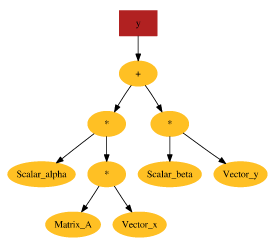
\includegraphics{img/DESOLA_running_example}
\par\end{centering}

\caption{\selectlanguage{english}%
\label{fig:Lib:DESOLA-DAG}\foreignlanguage{british}{An example DAG.
The rectangular node denotes a handle held by the library client.
The expression represents the matrix-vector multiply function y =
αAx + βy.}\selectlanguage{british}
}
\end{figure}


Figure \ref{fig:Lib:DESOLA-DAG} shows a tree, or more generally a
directed acyclic graph (DAG), accumulated during the evaluation of
a matrix-vector multiply function. The important thing to note is
that the authors insist on that DAG is a more effective way to record
computations than a tree as it exposes the sharing of {}``recipes''
among handles in the client code. This may not always be possible
in a purely functional context and will have to be explored. The actual
fusion algorithms employed in DESOLA are not explained in much detail.
The authors found that their achievements in fusion using the information
only available at runtime compensated the runtime code generation
cost for many real sized problems. The authors also believe that the
benefits of array contraction will be more noticeable once they add
support for sparse matrices and similar irregular data structures
to their library. As this is the focus of DPH, array contraction may
be beneficial to look at in more detail.

Overall, the approach of delaying the evaluation until it it required
seems promising and aligns well with Haskell's approach to lazy evaluation
(only from the ideological point of view, since the performance is
the first priority for DPH).


\subsection{Haskell Fusion Systems}

This section will review the previous approaches to fusion in Haskell.
It will cover Shortcut Fusion and DPH's very own Stream Fusion and
Functional Array Fusion.


\subsubsection{Shortcut Fusion}

Shortcut Fusion \cite{GLP93} is one of the most referenced techniques
for fusion in Haskell. It has been developed to be used in GHC to
fuse pipelined list operations. It employs two combinators, $foldr$
and $build$, and a single rewrite rule to eliminate adjacent occurrences
of the combinators. It is suitable for use in the cases when the functions
to be fused can be defined in terms of these combinators. $ $The
definition of $foldr$ is reused from Prelude, Haskell's standard
library:

\begin{lstlisting}[basicstyle={\ttfamily},language=Haskell]
foldr :: (a -> b -> b) -> b -> [a] -> b
foldr f z []     = z
foldr f z (x:xs) = f x z : (foldr f z xs)
\end{lstlisting}


To understand the motivation behind shortcut fusion one may think
of $foldr$ as of replacing each $Cons$ of a list with a binary operator
and $Nil$ with the neutral element. The other combinator, $build$,
takes a second order function which in turn takes an operator to be
used as $Cons$, and a value to be used as $Nil$. Since we are building
a list, these immediately become \texttt{(:)} and \texttt{{[} {]}}.

\begin{lstlisting}[basicstyle={\ttfamily},language=Haskell]
build :: ((a -> b -> b) -> b -> b) -> [a]
build g = g (:) []
\end{lstlisting}


To illustrate the approach a $map$ could be defined in terms of $build/foldr$
as follows:

\begin{lstlisting}[basicstyle={\ttfamily},language=Haskell]
map f xs = build (\c n -> foldr (c . f) n xs)
-- c is (:), n is []
\end{lstlisting}


In the above code the list is being folded into another list. With
the help of a rewrite rule

$\text{⟨}foldr/build\, fusion\text{⟩\,}\forall g\, k\, z.foldr\, k\, z\,(build\, g)\mapsto g\, k\, z$

the two consecutive $map$s could be reduced to as in the following:

\begin{lstlisting}[basicstyle={\ttfamily},language=Haskell]
map h (map f xs)
 -- inline
 = build(\c n -> foldr (c.h) n 
  (build (\c n -> foldr (c.f) n xs)))
 -- apply rewrite rule
 = build(\c n -> ((\c n -> foldr (c.f) n xs) (c.h) n)
 -- beta reduce
 = build(\c n -> foldr (c.h.f) n xs)
\end{lstlisting}


While this leads to the desired results in many cases, it requires
the programmer to define the functions in a not very readable form.
This may be acceptable for some of the code in the standard library
but is not likely to be widely accepted among client programmers.
Thus the fusion breaks for the parts of the code that do not use the
explicit $build/foldr$ definitions. To solve this, Chitil proposed
a type inference algorithm to automatically infer the $build/foldr$
definitions\cite{Chi99}.

Some of the other limitations of the Shortcut Fusion include the inability
to effectively fuse left folds and zips. These shortcomings make this
approach less attractive for DPH.


\subsubsection{Stream Fusion}

Stream Fusion \cite{CLS07,CSL06} is currently employed in the DPH
primitive library at one of the three levels of fusion discussed in
Section \vref{Lit:DPH-fusion-levels}.

It introduces two data types: a stream and a stepper. 

\begin{lstlisting}[basicstyle={\ttfamily},language=Haskell]
data Stream a = forall s. Stream (s -> Step s a) s
\end{lstlisting}


A $Stream$ is defined by its stepper function and seed. The stepper
is used to produce a stream by taking the current seed and yielding
the next step. That is, the stepper produces next element and state
from current state. The next step may be one of the following:

\begin{lstlisting}[basicstyle={\ttfamily},language=Haskell]
data Step s a = Yield a s
              | Skip s
              | Done
\end{lstlisting}


A $Done$ would flag the end of the stream, while $Yield$ would contain
an element and the next seed. If a $Skip$ is retrieved that would
mean that the current step does not contain an element. Thus streaming
of a list could be defined in the following way:

\begin{lstlisting}[basicstyle={\ttfamily},language=Haskell]
stream :: [a] -> Stream a
stream step0 = Stream next step0
  where next []     = Done
        next (x:xs) = Yield x xs
\end{lstlisting}


In the above the list itself is being used as the seed. Unstreaming
back to a list takes the following form:

\begin{lstlisting}[basicstyle={\ttfamily},language=Haskell]
unstream :: Stream a -> [a]
unstream (Stream next0 step0) = unfold step0
  where unfold s = case next0 s of
          Done       -> []
          Skip s'    -> unfold s'
          Yield x s' -> x : unfold s'
\end{lstlisting}


Any fusible list function should now be defined in terms of Streams
as opposed to lists, e.g.:

\begin{lstlisting}[basicstyle={\ttfamily},language=Haskell]
mapS :: (a -> b) -> Stream a -> Stream b
mapS f (Stream next0 s0) = Stream next s0
  where next s = case next0 s of
    Done       -> Done
    Skip    s' -> Skip        s'
    Yield x s' -> Yield (f x) s'

map :: (a -> b) -> [a] -> [b]
map f xs = unstream (mapS f (stream xs))
\end{lstlisting}


To see how a $Skip$ step might be used it may be worthwhile to look
at the definition of the $filter$ function.

\begin{lstlisting}[basicstyle={\ttfamily},language=Haskell]
filterS :: (a -> Bool) -> Stream a -> Stream a
filterS p (Stream next0 s0) = Stream next s0
  where next s = case next0 s of
    Done                   -> Done
    Skip    s'             -> Skip    s'
    Yield x s' | p x       -> Yield x s'
               | otherwise -> Skip    s'

map :: (a -> b) -> [a] -> [b]
map f xs = unstream (mapS f (stream xs))
\end{lstlisting}


The fusion opportunity such as $(map\, f\cdot filter\, p)$ may now
be exploited with the following rewrite rule

$\text{⟨}stream/unstream\, fusion\text{⟩}\,\forall stream(unstream\, s)\mapsto s$

In order to completely remove all traces of the helper data structures
Stream Fusion relies on general purpose compiler optimisations. This
makes this approach highly depended on GHC. However, due to the non-portability
of DPH this does not pose a problem. The major problem with this approach
is that the two primitive operations must be adjacent to each other
when inlined. This is not always possible. However, the approach is
very solid otherwise and it might turn out to be yet more effective
when combined with a runtime fusion system.


\subsubsection{Functional Array Fusion}

This last approach will be described by first developing an intuition
that would lead to the solution more thoroughly described in \cite{CK01,CK03}.
We will go to a greater depth describing this approach since it lays
down the basis for the work presented.

When talking about fusion it it important to do so with reference
to the context. In our case the interface to the primitive library
is limited by a number of predefined functions. This is contrary to
the approaches that optimising compilers take for fusing generic free-form
loops \cite{KA02}. Now that we have established that the interface
to the arrays is fixed it is worthwhile to consider the types of operations
it offers. Quite expectedly it follows some of the Haskell Prelude
conventions as well as the client interface to DPH (Figure \vref{fig:Lit:DPH-interface-functions}).

Suppose that one of the evaluation paths of the program arrives at
the following computation:

\begin{lstlisting}[basicstyle={\ttfamily},language=Haskell]
fold (+) 0 (filter isPrime (map (+1) (map (^2) (enumFromTo 0 9))))
\end{lstlisting}


The dependence graph \cite{RMKB06,KA02} for this computation is presented
on the left of Figure \vref{fig:Prime-Sum-evaluation}. One of the
ways in which the library functions can be classified is by the types
of their arguments and return types. We only focus on whether the
function produces or consumes array(s).

\begin{figure}
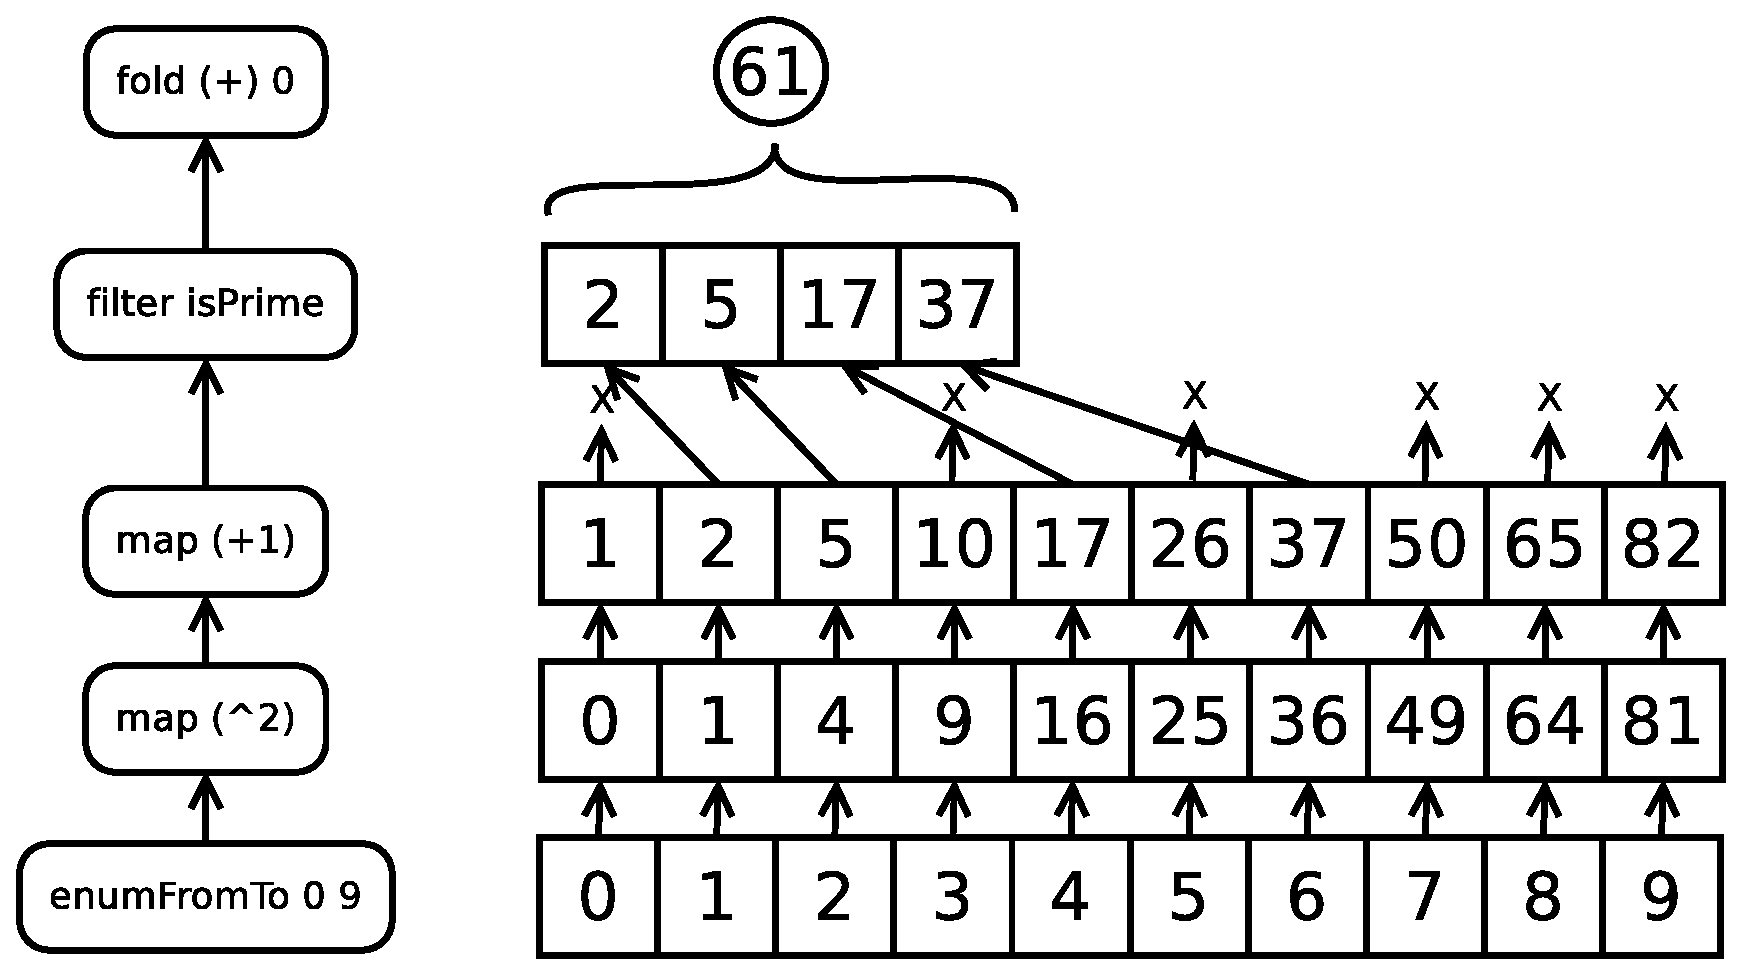
\includegraphics[width=1\textwidth]{img/SumPrimes}

\caption{\selectlanguage{english}%
\label{fig:Prime-Sum-evaluation}\foreignlanguage{british}{Prime Sum
evaluation tree. Delayed evaluation tree (left) and values at every
step (right).}\selectlanguage{british}
}
\end{figure}


In the above example we have an enumeration which always produces
and array but consumes none. This functions of this type are called
generators by the original authors. A more generic name for them is
anamorphisms {[}bananas{]}. These functions are used to bring arrays
into the scope of array operations.

The dual of anamorphisms are catamorphisms, or reductions, which consume
array(s) and only return scalar values. Folds are one example of such
functions.

Most of the functions in the library, however, are hylomorphism which
means they consume and produce at least one array. If fusion is not
used, each of such functions would allocate a new array and fill it
in before the next combinator consumes the newly created array. It
is desirable to avoid this. The way Functional Array Fusion looks
at this problem is it considers the computation as a pipeline of array
combinators, whereby each element is consumed in a lockstep and is
directly projected to the correct position in the resulting array.
As the right of Figure \vref{fig:Prime-Sum-evaluation} suggests,
each element is visualised as being \emph{mutated }in some way to
produce the final result. Thus, for each new element \emph{enumFromTo
}generates it is first squared, then incremented by one. It is then
run through the predicate of the filter and is taken into account
when folding to the final value if found to be true.

The way in which the original authors approached the problem was to
generalise generators, reductions and producer/consumers to a small
set of combinators covering most of the library interface. They came
up with the \emph{loop} combinator of the following type (adjusted
to be consistent with the rest of this document):

\begin{lstlisting}[basicstyle={\ttfamily},language=Haskell]
loop :: (e -> a -> (Maybe e', a)) -- mutator function
     -> a                         -- accumulator
     -> Array e                   -- input array
     -> (Array e', a)
\end{lstlisting}


The \emph{loop }combinator traverses the input array \emph{arr}. The
mutator function is made generic so as to be able to act as function
supplied to \emph{map}, \emph{filter} and \emph{fold} combinators.
Thus, \emph{map f} can be implemented as \emph{loop }with a unit accumulator
and the following mutator function:

\begin{lstlisting}[basicstyle={\ttfamily},language=Haskell]
map_mf :: (e -> a -> (Maybe e', a))
map_mf x acc = (Just (f x), acc)    -- acc unused
\end{lstlisting}


Similarly, \emph{filter p }and \emph{fold f acc }can be implemented
as \emph{loop}s\emph{ }with the following mutator functions:

\begin{lstlisting}[basicstyle={\ttfamily},language=Haskell]
filt_mf :: (e -> a -> (Maybe e', a))
filt_mf x acc = (filt, acc)         -- acc unused
  where filt = case (p x) of
                 True  = Just x
                 False = Nothing

fold_mf :: (e -> a -> (Maybe e', a))
fold_mf x acc = (Nothing, f x acc)  -- no elt produced
\end{lstlisting}


It should be noted from the above that the \emph{loop }combinator
is able to express both hylomorphisms (\emph{map, filter}) and catamorphisms
(\emph{fold}). The latter are identified by the \emph{Nothing }value
unconditionally returned by the \emph{mutator function. }The only
function from the original example that is left to be defined in terms
of the \emph{loop }combinator is the anamorphism \emph{enumFromTo.}
Its mutator function might%
\footnote{The library implementation generalises enumerations to \emph{enumFromStepLen},
which takes a value for the first element, the increment and desired
length of the resulting sequence.%
} take the following form:

\begin{lstlisting}[basicstyle={\ttfamily},language=Haskell]
enum_mf :: (e -> a -> (Maybe e', a))
enum_mf _ acc = (Just acc, acc+1)   -- acc is next val
\end{lstlisting}


The above implementation of \emph{enum }suggests that it might be
possible to express generators using the generic \emph{loop }combinator.
However, a careful reader may have noticed that \emph{loop, }by definition,
traverses \emph{an array}, even though the value of the element is
ignored in this particular mutator function. Thus, a cheap but generic
implementation of generators would have been possible if we had a
dummy array to iterate over. As discussed previously in \subref{DPH-Data-Repr}\vpageref{sub:DPH-Data-Repr}
an array of units can be represented by a single value -- its length.
Indexing the array at any position within the bounds would just return
a unit value%
\footnote{In Haskell a Unit type conveniently represented in source code as
\emph{() }is similar to a \emph{void }in C.%
}. Now, a generator like \emph{enumFromTo} could be easily and cheaply
implemented as follows:

\begin{lstlisting}[basicstyle={\ttfamily},language=Haskell]
enumFromTo :: Int -> Int -> Array Int
enumFromTo start end = fst (loop enum_mf start units)
  where units = replicate (end - start + 1) ()
\end{lstlisting}


In the above implementation an array of units is first constructed
by replicating (repeating) a unit value the desired number of times.
It is then traversed using the appropriate mutator function resulting
in a tuple with the desired enumeration in the first position and
the final accumulator in the second (\emph{end+1} in this case). We
can safely drop the accumulator as we are only interested in the array.

The true convenience of the \emph{loop }combinator is revealed if
we try to squash multiple \emph{loop }combinators into a single \emph{loop}.
GHC's rewrite rules mechanism is employed to pipeline two adjacent
\emph{loop}s. For the sake of being concise we will omit here most
of the infrastructure required for the approach to work. We present
the way by which two mutator functions can be merged into a single
one:

\begin{lstlisting}[basicstyle={\ttfamily},language=Haskell]
-- mutator function of the first loop
mf1 :: e0 -> a1 -> (Maybe e1, a1)

-- mutator function of the second loop
mf2 :: e1 -> a2 -> (Maybe e2, a2)
\end{lstlisting}


\begin{lstlisting}[basicstyle={\ttfamily},language=Haskell]
-- mutator function to express
-- loop mf2 .. (loop mf1 .. (..)) as a single loop
mf :: e0 -> (a1,a2) -> (Maybe e2, (a1,a2))
mf x (acc1, acc2) =
  case (mf1 x0 acc1) of
    (Nothing, acc1') = (Nothing, (acc1', acc2))
    (Just x1, acc1') =
      case (mf2 x1 acc2) of
        (Nothing, acc2') = (Nothing, (acc1', acc2'))
        (Just x2, acc2') = (Just x2, (acc1', acc2'))
\end{lstlisting}


Since the mutator function may not always return a value (e.g. in
the case with \emph{filter} combinator) merging two mutator functions
proceeds in two steps:
\begin{enumerate}
\item We first run the given array element through the first mutator function.
If that does not produce a value (produces a \emph{Nothing}) we do
not proceed to the second mutator and yield \emph{Nothing }as the
overall result.
\item In case the first mutator did produce a value (\emph{Just}) we run
it through the second mutator, returning the final result whatever
it might be.
\end{enumerate}
Clearly, some trickery is involved in dropping the first accumulator
in a (potentially deeply nested) pair, but the above conveys the main
concepts behind the Functional Array Fusion.


\subsection{Summary}

This section has reviewed some of the array fusion frameworks covering
a number of:
\begin{itemize}
\item languages (C++, Haskell),
\item applications (algebraic libraries, general purpose list library, data
parallel framework),
\item approaches (runtime evaluation graph optimisation, equational fusion
based on rewrite rules).
\end{itemize}
The discussion in the next section will be based on the fusion frameworks
described above.

\pagebreak{}


\section{Proposal}

The current project is carried out completely within the context of
the Data Parallel Haskell project. Therefore, the fusion frameworks
designed specifically for Haskell were the first to turn to. The Background
section discussed three of them: Shortcut Fusion, Stream Fusion and
Functional Array Fusion. Glasgow Haskell Compiler's rewrite rules
functionality plays crucial rule in all three of them. This is not
coincidental:
\begin{itemize}
\item Compile-time term rewriting is fundamental optimisation technique
in the implementation of functional programming languages \cite{Pey87}.
Exposing it to the user \cite{PTH01} makes it an attractive way to
expose compiler functionality to pure library code
\item Inlining \cite{PM02} is another technique which is crucial in compilers
like GHC which heuristically removes superfluous levels of indirection
in the original code. As a side effect it provides more opportunities
for term rewriting to happen
\item Haskell is a purely functional language therefore valid term rewriting can be
done without a sophisticated analysis of side effects. Rewriting would
generally be unsafe in a non pure context
\item (In the case with Stream Fusion) it is reasonable to rely on the existence
of certain compiler optimisations since DPH relies on GHC and is not
designed for other Haskell implementations
\end{itemize}
The above statements suggest that compile time equational fusion seems
like a natural choice for the Haskell programming language. This is
especially valid for Stream Fusion where the authors were able to
achieve, through inlining, rewriting and compiler optimisations, the
speed of handwritten code. Moreover, the generated code for many examples
was the same as a human programmer would normally write. However,
the strong dependence on the optimisation systems of such a complex
system as GHC makes the fusion frameworks fragile and non-portable.

One of the cases in which fusion breaks is when two array operation
do not end up being adjacent after inlining. This may happen due to
the so called \emph{let floating }optimisation in GHC \cite{PPS96}.
This optimisation is designed to avoid duplicating work. When GHC
finds two identical terms in an expression and considers them large
enough to benefit from computing them only once, it \emph{floats}
them out to a new \emph{let }binding outside of the expression. This
optimisation is the opposite of inlining. If the term that was forcibly
floated out would have otherwise completed a pattern for a fusion
rule, that fusion opportunity is missed.

The other problem with equational fusion is that \emph{sharing }is
not clearly defined. This is related to the above problem. Sharing
prevents large amounts of work to be duplicated. Aggressive unconditional
inlining would have introduced a major inefficiency for programs in
which the result of a pipeline of costly array operations is independently
used in more than on place. Recomputing the shared portion may result
in a noticeable performance hit.

Both of the above two problems suggests that correct inlining plays
a major part in the process of fusion. It also suggest that the decisions
taken by the inliner do not always result in the optimal code for
exploiting fusion. 

One of the goals of the current work is to reduce the dependency of
successfully exploited fusion opportunities on the behaviour of the
inliner. It was decided to explore the possibility of performing fusion
at runtime of the program. That would eliminate the need for the inliner
at least for the part of decision making when fusing array operations
together. The DESOLA library, while designed for C++, serves as a
starting point for performing fusion at runtime. The new framework
would reuse its approach of constructing a dependence tree. When an
array computation is later forced by a catamorphism, the tree can
be optimised yielding an equivalent computation in a fused form.

The very first design decision to make would be the way to represent
delayed array operations as nodes in the tree. Haskell's ability to
delaying function application and effortless function composition
to create new functions has lead the author to reusing the approach
of Functional Array Fusion. Thus each node in the tree could be:
\begin{enumerate}
\item A handle to a \emph{loop }based computation for which we store an
appropriate mutator function, the initial accumulator value and the
parent node in the previous node in the tree
\item Alternatively, it could be a handle to a delayed replication, i.e.
an array of a given length which has the same value in each position
\end{enumerate}
The tree represented in this manner may be flattened at any time to
a replication handle, call it \emph{ReplicateH} wrapped in a loop
handle, \emph{LoopH}. All of the library's interface functions can
then be implemented in terms of the handles to the delayed tree operations.
As a special case, the catamorphic functions, not only obtain a new
delayed array handle but also force the evaluation of the tree.

The next feature of the new framework to be implemented would be the
support for segmented array operations. Segmented array operations
are central to DPH. Implementing them would complete the interface
of the library. Luckily the authors of Functional Array Fusion have
provided one solution for it. Implementing it would require modifying
the the type signature of the mutator function and generalising the
\emph{loop }combinator to support segment boundaries.

The next major feature required for DPH to be used with the new backend
as intended would require adding support for distributing computations
over the available processing elements. At present time DPH has two
backends: one purely sequential and one parallel. However, they are
not entirely independent. The parallel backend is concerned with only
the following:
\begin{itemize}
\item splitting (chunking) arrays and distributing them among a \emph{gang
of threads}
\item calling a sequential implementation from the sequential backend on
each chunk
\item joining the chunks from the finished parallel operations
\item statically removing as many synchronisation points as possible (split-joins) 
\end{itemize}
The last item on the list was parallel backend's own fusion system
described \vpageref{Lit:DPH-fusion-levels}. Fusion in the sequential
backend occurs only after that in the parallel backend (more precisely
after a split and before the next join). On one hand that allows the
two fusion systems to be independent. However, considering the nature
of the new sequential backend it may sometimes do no work between
the two split-joins. Indeed, we said initially that we were only forcing
the evaluation of the tree when reaching a catamorphism. A dynamic
technique for eliminating superfluous synchronisation points in the
context of functional programming languages has been suggested in
{[}Operator fusion{]} under the name Operator Fusion for the Scala
programming language. It is a simple algorithm with requires every
function in the library to be classified according to:
\begin{itemize}
\item whether or not the inputs are consumed sequentially (\emph{map} vs.
\emph{backpermute}),
\item whether or not the outputs are produced sequentially (\emph{map} vs.
\emph{permute}),
\item whether or not load unbalancing may happen (\emph{map} vs. \emph{filter})
\end{itemize}
While the \emph{loop }operator presumes traversing the array from
left to right, the aforementioned work may prove to be useful when
adjusting the parallel backend.

Lastly, there are two optional features that may be researched and
possibly implemented:
\begin{enumerate}
\item Traversing more than one array\emph{ }one after the other, e.g. using
\emph{concat }or \emph{concatMap}
\item Sharing recovery and fusion preserving sharing. Normally, it is not
possible in the purely functional context to refer to the same tree
node from two other nodes to share computation between them. Turning
the tree into a Directed Acyclic Graph (DAG) to enable sharing would
require extra effort. This problem has been researched in the context
of Accelerate Domain Specific Language embedded in Haskell \cite{CKL+11}.
Fusion preserving sharing is a step up from sharing recovery enabling
to continue running running multiple computations in a fused manner
(as opposed to first precomputing the shared portion of the DAG).
\end{enumerate}
\pagebreak{}

%%%%%%%%%%%%%%%%%%%%%%%%%%%%%%%%%%%%%%%%%%%%%%%%%%%%%%%%%%%%%%%%%%%%%%%%%
\section{LiveFusion}

\subsection{Delaying computation: LiveFusion AST}

In its essence LiveFusion take the approach of deeply embedded domain specific languages (EDSLs). The principle idea of deep embedding is the introduction of its own abstract syntax tree (AST) which is separate from the host language AST but is rather presented as a tree structure in the host language. The difference with the AST found in compilers is that it allows one to analyse, optimise and compile or interpret the EDSL's AST at runtime using the host language in the library code, withought the difficulties of writing a complete standalone optimising compiler. The added benefit of the approach is that the EDSL code can interact with the other code in the language.
\begin{comment}TODO separate EDSL discussion from deep embedding\end{comment}

The fundamental concept by which LiveFusion makes fusion possible is constructing an AST of pending array operations at runtime and compiling that AST to fast code when the result in required in the host program. An AST defined in the host language (Haskell in this case) is what makes the delaying of computations possible. It is the topmost layer of LiveFusion system in that most of the library's user-facing combinators discussed in Section \begin{comment}TODO\end{comment} are for the most part just constructing the nodes of the AST. This way an AST representing the core of QuickHull example discussed previously becomes the following (TODO figure ref).

\begin{lstlisting}[basicstyle={\ttfamily},language=Haskell]
farAndAbove :: (Point,Point) -> Array Point -> (Array Point, Point)
farAndAbove line points
  = let distances = map (dist line) points

        -- Find maximum point
        indexed     = zip (indices distances) distances
        farthest_ix = fst $$ fold maxSnd 0 distances
        farthest    = points !! farthest_ix
        maxSnd x y  = if snd x >. snd y
                      then x
                      else y

        -- Find all points above the line
        positive    = map (>. 0) distances
        above       = packByTag positive points

    in  (above, farthest)
\end{lstlisting}

\begin{comment}INSERT FLAT QH AST FIGURE HERE\end{comment}

The above example uses six aray combinators: $map$, $zip$, $indices$, $pack$, $fold$ and the indexing combinator $!!$. The first four of them are $array transducers$ in that they both consume and produce arrays. On the other hand $fold$ and $!!$ consume arrays and return a scalar value, so we call them pure consumers.

It is now time to show the AST node constructors these combinators correspond to. LiveFusion AST is a Generalised Algebraic Data Type (GADT) (TODO cite) whose individual constuctors correspond to delayed array operations. In principle, given an interpreting function such as $eval :: AST t -> t$ an value of type $t$ encoded in the $AST$ language can be computed. Nowhere does it specify that $t$ is an array. In fact we know not all of the array combinators return an array: it has been discussed that $fold$, $!!$ and several others return a scalar value. To express the dimensionality of the result we introduce $type ArrData a$ which in our implementation is represented by $Vector a$ from $vector$ package (TODO ref). We introduce type synonyms $ArrayAST a$ and $ScalarAST a$ to distinguish between the two.

\begin{lstlisting}[basicstyle={\ttfamily},language=Haskell]
type ArrayAST a = AST (ArrData a)
type ScalarAST a = AST a

data AST t where
  Map      :: (Elt a, Elt b)
           => Exp (a -> b)
           -> ArrayAST a
           -> ArrayAST b

  Zip      :: (Elt a, Elt b)
           -> ArrayAST a
           -> ArrayAST b
           -> ArrayAST (a,b)

  Fold     :: Elt a
           => Exp (a -> a -> a)
           -> ScalarAST a
           -> ArrayAST a
           -> ScalarAST a

  PackByTag :: Elt a
            => ArrayAST Bool
            -> ArrayAST a
            -> ArrayAST a

  Indices  :: Elt a
           => ArrayAST a
           => ArrayAST Int

  Index    :: Elt a
           -> ArrayAST a
           -> ArrayAST Int
           -> ScalarAST a
\end{lstlisting}

\subsection{Parametrising higher-order functions}

Another notable feature of the interface to note here is the type of functions parametrising the higher-order combinators like \texttt{map} and \texttt{fold}. They are all of the form \texttt{Exp (a -> b)} or \texttt{Exp (a -> a -> b)}. The corresponding functions in Haskell Prelude or array libraries like \texttt{Vector} or \texttt{Repa} accept as arguments simple Haskell functions like \texttt{a -> b} or \texttt{a -> a -> a} as long as the types match. So why cannot LiveFusion be the same? The answer lies in the approach to evaluating the AST. LiveFusion AST is open to interpretation by several backends as discussed in Section (TODO ref), and the currently supported one includes the compilation step. When using this backend, the AST is compiled to one or more loops for which Haskell code is generated and written out to file. If the parametrising functions were simple Haskell functions, they would have be compiled to machine code before the program is run. When the AST is later constructed at runtime they would only be available in form of closures which can be called but not inspected\footnote{There is a non-portable way to explore closures in Haskell, but it will not allow one to easily make use of the code compiled to binary. See discussion in Section (TODO ref)}. Suppose the user calls \texttt{map (+1) xs}. The mentioned array libraries rely on the function \texttt{(+1)} being inlined into the compiled loop code to produce efficient code. If this does not happen, calling \texttt{(+1)} for every element in the array will result in the following:
\begin{enumerate}
\item Boxing the element value by placing it in the heap
\item Calling the closure with the pointer to the boxed value
\item Jumping to the address of the \texttt{(+1)} function referenced in the closure
\item The code will unbox the value, increment it and create a new value on the heap
\item The loop code will then need to unbox the result and write it into the result array
\end{enumerate}

This is a very round-about way of incrementing a value in a tight loop and will greatly affect the performance of the loop. Unfortunately, at the time of generating code for AST, all these haskell functions will have been compiled to machine code and be only available as closures. There is currently no way to inline them or get the original Haskell source code from which they were created. We needed to find a way to generate efficient code for user specified functions at runtime.

Thus, we need a way to record the user-provided functions in a more high level way than machine code. In summary our representation for functions:
\begin{enumerate}
\item Provides backend independent interface offering many common functions
\item Allows backend-specific implementation for each function
\item Hides implementation from the user by default
\item Allows user to compose functions in a way that looks very native
\item Allows user to provide direct backend-specific implementation for new functions that cannon be composed from functions already provided
\end{enumerate}

%% Does Accelerate fix the primitive functions as constructors in an ADT?

So what is \texttt{Exp (a -> b)}? It is a term in our scalar expression language $Exp$, representing a function from type $a$ to type $b$:
\begin{lstlisting}[basicstyle={\ttfamily},language=Haskell]
data Exp t where
  -- Literal or non-function value
  ConstE :: a -> Exp a

  -- Function implemented in the backend
  FunE :: Impl t -> Exp t

  -- Lambda abstraction
  LamE :: (Exp s -> Exp t) -> Exp (s -> t)

  -- Function application
  AppE :: Term (s -> t) -> Term s -> Term t
\end{lstlisting}

(TODO discuss HOAS and distinction between function values and non function values)

(TODO discuss Exp and HOAS, for now skipping to Impl)

The notable part of the \texttt{Exp} language is its constructor \texttt{FunE}. The only argument to the constructor is \texttt{Impl t} which is a backend-dependent way of defining a function. \texttt{Impl} gives freedom to the backend to choose the most suitable representation for a function. For instance, in out Haskell backend, we are interested in generating Haskell source code, for which \emph{Template Haskell} (TODO ref) is a natural choice. Thus we choose the following definition of \texttt{Impl}:
\begin{lstlisting}[basicstyle={\ttfamily},language=Haskell]
data Impl t = HsImpl {
                hs :: t,        -- Native Haskell function
                th :: Q TH.Exp  -- TemplateHaskell quasiquoted expression
              }
\end{lstlisting}

The Template Haskell expression is really the core part of the function representation, but this is what whould later on allow us to produce Haskell source code without much trouble. We also include simple Haskell function with our representation. At present this is just for completeness. However in the future it may be possible to avoid compiling certain parts of AST at runtime and run statically scheduled combinators. In this case this whould be the function to inline in the loop.

We will now show the (rather trivial) implementations for a couple of functions before continuing with our explanation of Impl.

\begin{lstlisting}[basicstyle={\ttfamily},language=Haskell]
plusImpl :: Num a => Impl (a -> a -> a)
plusImpl = HsImpl { hs = (+); th = [| (+) |] }

absImpl :: Num a => Impl (a -> a)
absImpl = HsImpl { hs = abs; th = [| abs |] }
\end{lstlisting}

It is easy to see that TemplateHaskell expressions are trivially created from simple Haskell functions using QuasiQuotation syntax (TODO ref). When the backend is ready to generate Haskell source for these functions, it will be a simple matter of using a pretty printer. The reasons for using TemplateHaskell instead of strings in the first place when the conversion is so trivial are the following:
\begin{itemize}
\item The backend does more than trivial code generation as discussed in Section (TODO ref), where the full power of TemplateHaskell is required. Functions defined via TemplateHaskells become very easy to incorporate into the syntax tree being generated
\item New developments in TemplateHaskell\footnote{Starting with GHC 7.8.} will allow its expressions to be typed. Having \texttt{Q (TExp t)} as opposed to \texttt{Q Exp} will provide an extra layer of safety to our function representation
\end{itemize}

\subsubsection{Other backends and more backend functionality}
\begin{itemize}
\item Currently function representation of only one backend was shown, namely Haskell source backend.
\item Even that one was trivial: only containing a TH Exp + native HS function
\item What other functionality may we want in our function representation?
\item LiveFusion is a fast array processing library. The focus is on performance.
\item Our two main options for speed on modern CPUs: parallelism + vector instructions.
\item Parallelism is already exploited by DPH through other means and will split the computations evenly across all cores
\item Vectorisation on the other hand has not been exploited by DPH yet\footnote{Though new developments in that area have emerged more recently [TODO ref].}
\item The CPU manufacturers are introducing and announcing more and more vector instruction sets \footnote{TODO Ref: Intel Future Instruction Sets} which will allow many types of vector operations to be performed on each core.
\item This is very handy for libraries like LiveFusion which are already providing patterns of array computation, some of which map very well to vector instructions of current or future CPUs (TODO find examples, but this will definitely include pointwise arithmetic, reductions and pack).
\item At some point in the future \texttt{Impl} function representation may be the most natural place to include backend- or even CPU-specific information, on how to generate vector instructions for a particular function, e.g. a reduction using product operator on an Intel CPU.
\end{itemize}

\subsubsection{User provided backend implementation}

One feature of the given scalar functions representation allows the user to provide implementation of arbitrary functions the way they want the backend to generate them. After all, it only requires creating a new record of type \texttt{Impl t} where \texttt{t} is the type of the desired function. Library user can then provide the internals of function implementation to appear in the generated code.

This functionality may seem unneccessary, since the library already provides all functions from such type classes as \texttt{Num}, \texttt{Ord}, \texttt{Floating}, etc., as well as a powerful mechanisms to compose them into more complex functions. However, in the light of vector instructions discussion in Section (TODO ref), leaving this door open to the user may be valuable and make the library more flexible on more architectures.

%%\begin{itemize}
%%\item Closest to the API
%%\item User-facing arrays are internally represented a ASTs.
%%\item Give example
%%\item What does AST need to keep track of
%%\item Show the data structure
%%\item A deeply embedded EDSL
%%\item Creates an internal AST of type \texttt{AST a}, which represents a delayed computation returning \texttt{a}.
%%\item LiveFusion is an array processing system, so our main type is an array, say \texttt{Vector a}. Thus a delayed computation returning a \texttt{Vector} of element of type \texttt{a}s would be represented as \texttt{AST (Vector a)}
%%\item But vectors are not the only data type we can handle, hence we can also have \texttt{AST (Int, Float)} - a delayed computation, which, when forced, produces a pair of an \texttt{Int} and a \texttt{Float}.
%%\end{itemize}


\subsection{Sharing recovery: Abstract Sematic Graphs}
\begin{itemize}
\item Find example, should be plenty in QuickHull
\item Talk about ref transparancy of Haskell
\item While can still fuse, it performs unneccessary work
\item Still represented by the same object internally at runtime
\item StableNames, Gill's, but can do other
\item It's is IO, but since we are in a library and can guarranty safety by design we don't care
\end{itemize}

\subsection{Retreiving the result}
\begin{itemize}
\item LiveFusion delayed computations live in its own data type.
\item 
\end{itemize}

\subsection{Loop representation: Loop Language}
\begin{itemize}
\item inherently procedural
\end{itemize}

\subsubsection{Communication by Convention}
\begin{itemize}
\item Many of the combinators use a similar set of variables, e.g. both Map and Scan produce a value at each iteration which they assign to an intermediate variable in the body of the loop, say elt
\item Thus if there are two maps one after the other, we need to distinguish between the two
\item We give earch such variable a unique identifier which coincides with the identifier of the combinator in the graph (see section), e.g. $elt_3$ is always an intermediate element produced by combinator 3 in each iteration (provided the combinator is a producer)
\item Other examples include $len_1$, $i_1$, $o_5$, $acc_4$
\item Not only this removes any potential name clashes (since ids are unique), but also allows us to refer to any variable in the loop just knowing what function it's performing as well as the combinator id.
\item When is it useful? Can we have a DS passing those variables without stupid conventions?
\item The problem is that the names are generated by convention, so in case of any error, the program would either fail to compile at runtime or produce incorrect results
\item The easiest way 
\item Like global variables
\item Spooky action at a distance
\item Untracked interaction between different parts of loop
\item In many cases a flaw of software design, often discouraged and even semantically prohibited in functional languages like haskell and ml.
\end{itemize}


\subsection{Procedural code: Imperator Language}

%%%%%%%%%%%%%%%%%%%%%%%%%%%%%%%%%%%%%%%%%%%%%%%%%%%%%%%%%%%%%%%%%%
\subsection{Code generation and loading}

Ways (haskell, external (c), llvm)

\subsubsection{Haskell code generation}

\subsubsection{What do we need to generate}
\begin{itemize}
\item
\end{itemize}

\subsubsection{Efficient numeric computations in Haskell}
\begin{itemize}
\item Talk about haskell data structures (lists, arrays)
\item about boxed values
\item Prohibitive performance costs
\item Unboxed values
\end{itemize}

\subsubsection{Mutable vectors}
\begin{itemize}
\item Very low level access
\item Haskell vector or GHC.Prim
\item Largely the same underneath
\item Vector may be more intuitive
\item Offers many types of vectors and levels of access to them
\item Uses ST monad, to make sure...
\end{itemize}

\subsubsection{Looping}
\begin{itemize}
\item There are many ways a loop can be represented in code
\item FPrs see it as a recursive function
\item Procedural programmers see it as a while or for C loop
\item Down at the machine level is a chunk of code with a label and jump statement to the beginning of the loop (or alternatively out of the loop)
\item When generating HsCode only rec fun, however want fast machine code in the end
\item Tail rec
\item Give example of what machine code it becomes
\item Thus need to make sure we always have tail rec
\end{itemize}

\subsubsection{Tail recursion}
\begin{itemize}
\item Perhaps put the points from above here
\end{itemize}

\subsubsection{Strictness}
\begin{itemize}
\item What is it and why
\item Strictness analysis example
\item Where in our case it would fail
\item What to do: two things, the easiest is !
\end{itemize}

\subsubsection{Inlining}
\begin{itemize}
\item Funcall costs
\item Perhaps give an example with benchmark
\item LLVM helps?
\end{itemize}

\subsubsection{Unboxing}
\begin{itemize}
\item Give example
\item Rewrite \texttt{case i\# of I\# ->} which rewrites
\end{itemize}


\subsubsection{Compilation and loading}

\subsubsection{Impedance matching}

\subsubsection{Unboxing}

\subsubsection{Performance considerations}

\subsubsection{Two types of sharing}
\begin{itemize}
\item Diamond is easy is there are many ways of achieving it, even though it compromises referential transparency. But we guarranty correctness by design. Extensively covered in section \ref{}
\item Problem arises if the diamond does not form before the result is required in one of the branches
\item Illustrate with QuickHull example
\item Would be less of a problem if we were analysing a static tree in the compiler since there are no conditionals so such a computation would always be there
\item However, when it comes to runtime we are limited by the execution order. If a result is required in Node x in Figure, then Node y won't be forced since none of the predeccessors of Node x know about the branch leading up to Node y.
\item This wouldn't be a problem in a language with mutable references, where the parents of the tree could know about its children
\item This has two censequences:
\begin{itemize}
  \item Even though the results of Node x and y can be computed in one loop, Node x will be computed first, thus a fusion opportunity is missed
  \item A bigger problem, however, is that it may lead to duplicated work
  \item Consider Node z when the branching occurs. At the time of computing Node x, the computation in Node and all of its predessessors will be fused into the loop computing result for Node x. Once the result of Node y is finally required, the coputation would have to start from scratch and include Node z and all of its predeccessors.
  \item In this case it would have been beneficial for performance to create an intermediate array at Node z and start the computation of Node y with that.
\end{itemize}
\end{itemize}

\subsubsection{One solution for branched sharing}
\begin{itemize}
\item It maybe benefitial to take a step back and think about the problem in terms of the data structures that represent the delayed computations
\item Trees
\item In general in Haskell trees the parents know about the children, but the children do not know about the parents. In the case of LiveFusion with predessessor in the pipeline of combinators is the child, while the root of the tree is the last combinator in the pipeline.
\item If we employ the common sharing recovery techniques, we get a graph in which the shared nodes are not repeated.
\item The important thing to note is that we still have a graph with ONE SINGLE root node. The same node that was the tree before sharing recovery.
\item The problem with branched sharing is that even before the sharing recovery takes place, we have not a tree but a graph. There are multiple tree roots (e.g. x and y) that are held by different parts of the program which happen to share some nodes.
\item Knowing about other such roots from at each one of them presents the essence of the problem we are facing
\item Here we present a sample solution to the problem which is set outside the LiveFusion framework
\item Describe that ugly sharing recovery example I wrote
\end{itemize}


\subsubsection{Delaying computation of scalar results}
\begin{itemize}
\item So far assumed that we have arrays as results
\item However, as discussed we distinguish three types of array combinators:
\begin{itemize}
  \item anamorphic combinators (generators)
  \item hylomorphic combinators (producer/consumers)
  \item catamorphic combinators (pure consumers)
\end{itemize}
\item A particular example of the pure consumets is a Fold and it produces a single scalar value- 
\item It is important to note the result type of function \texttt{fold}. It is just the element type. Compare it to the combinators which have the result type of Array a which is a synonym for \texttt{AST (Vector a)}. The latter clearly stately it is a delayed computation. However, in the case of $fold$ nowhere in the type singnature does it say it's a delayed computation.
\item The reason for this is in the way DPH integrates into Haskell
\item Arrays are library defined, while the scalars are Haskell built in.
\item Another way to look at it is if AST was the type of a typical EDSL. All array producing computations in LiveFusion are represented in this AST language. In much the same way Accelerate languare has Acc Array. However, unlike DPH, Acclerate also offers scalar computations and even functions represented as \texttt{Acc}: e.g. \texttt{Acc Int} and \_?\_ \texttt{(Int -> Int)} respectively.
\item Thus the type of fold would in Accelerate would look like ...
\item Due to the tighter integration of DPH with Haskell, it by design uses Haskell types directly, hence the type of the fold which uses haskell primitive types
\item This poses a problem that it forces the computation as soon as the reduction is reached as there is no data structure to hold the delayed computation in
\item This is usually the desired result, unless it is an instance of branched sharing discussed previously (outline an example)
\item There is currently no solution for the problem, however, for easier integration into other systems, LiveFusion does delay scalar computations, i.e. the type of Fold combinator is actually \texttt{..... -> AST a}. In fact the only thing that the wrapper \texttt{fold} functions does is: \texttt{fold f z xs = compute \$ Fold f z xs}
\end{itemize}

\subsubsection{Code reuse}
\begin{itemize}
\item Most of DPH programs are recursive in one form or the other.
\item E.g. QuickHull, NBody, etc..
\item In QuickHull ...
\item In NBody ...
\item The same graph of combinators are executed over and over again at each recursion step
\item Ammortising the cost of code generation and runtime code compilation and loading over a number of iterations is not a new problem in Computer Science [...refs...]
\item This problem has also been solved by the Accelerate EDSL for GPU programming in Haskell, so can be adapted.
\end{itemize}

\subsection{Discussion}

\subsubsection{What DPH gives up}
\begin{itemize}
\item Lots of Filtering (common FP approach)
\item Same length zipping
\item No unbounded lengths
\item
\end{itemize}

\subsubsection{Use patterns}
\begin{itemize}
\item Find them in examples
\end{itemize}


%%%%%%%%%%%%%%%%%%%%%%%%%%%%%%%%%%%%%%%%%%%%%%%%%%%%%%%%%%

\section{Planning}

In the previous sections we reviewed several approaches to array fusion.
We proposed a new approach to runtime fusion based on Functional Array
Fusion previously applied in DPH. It also uses ideas from the DESOLA
library to turn an equational array fusion framework into a runtime
one.

To initiate the discussion it would be appropriate to recall the original
problem any fusion system attempts to solve. In the beginning we said
that fusion transforms a high level program to one that approaches
the semantics and performance of a low level handwritten program.
The authors of Stream Fusion framework have found that Functional
Array Fusion was not up to the speed of their system even in the cases
where all of the fusion opportunities have been exploited by both
system \cite{CSL06}. They suggest that this is due to the overhead
introduced by the Functional Array Fusion framework. In is important
to note that both frameworks benefit from such compile-time optimisations
as inlining and term rewriting. However, when we turn a compile-time
to a run-time fusion none of these optimisations are available, so
at runtime we end up with unoptimised loops with function closures
and boxed values. It is clear that a fusion system would not be useful
if it exploits more opportunities yet introduces a large constant
factor minimising the positive effects. In other words it would not
be appropriate to transform one major problem into another.

There are eight major milestones two of which are optional and will
depend on the actual time spent on other tasks. The remainder of the
project is spanned across a period of 24-36 months ending with a thesis
submission. The following is the detailed descriptions of the tasks
depicted on the chart:
\begin{description}
\item [{1.\ Delayed\ sequential\ evaluation}] will require providing
a basic tree structure and simple \emph{loop} combinator implementation.
It must provide means for flattening the tree and evaluating it to
a final result. Primitive library functions that do not use segmentation
can now be implemented in terms of the delayed tree handles {[}completed{]}
\item [{2.\ Efficient\ loop\ combinator\ implementation}] will require
implementing the \emph{loop }combinator in terms of unboxed arrays.
Preliminary benchmarking can be done at this stage {[}completed{]}
\item [{3.\ Performance\ tuning}] will require optimising the new framework
to reduce the overhead associated with bringing fusion into runtime.
Preliminary results have been collected by running programs fused
by hand with the potential of a runtime fusion system in mind. They
show a performance improvement of up to 30-50\% in real world applications,
compared to the current Stream Fusion. This majour objective includes
adding support for runtime code generation, compilation and dynamic
loading. Preliminary tests show the necessity in the research of polyvariadic
functions and automating argument/return values unboxing
\item [{4.\ Sharing\ recovery}] is an non-optional task highly important
for high performance. Where conditional inlining would prevent Stream
Fusion from duplicating the work, a runtime fusion system such as
ours would collect all of the operations into one tree. This may lead
to duplicate subtrees which my be difficult to identify in a purely
functional context. An appropriate sharing recovery mechanism would
allow us to surpass the Stream Fusion system in many real world DPH
programs
\item [{5.\ Segmented\ sequential\ evaluation}] will require extending
the tree representation and the \emph{loop }combinator to support
segmentation. Previous work on Functional Array Fusion is likely to
be of help. Adding support for segmented evaluation will complete
a major part of all functions in the primitive library. This would
allow to benchmark real DPH programs (i.e. on irregular data structures).
\item [{6.\ Delayed\ parallel\ evaluation}] will require adding support
for true parallel evaluation. This would allow DPH to be used as intended,
automatically parallelising tasks across the available processing
elements
\item [{7.\ Traversing\ multiple\ arrays}] would allow the framework
to cover more of the library's array operations. While this is not
a task of immediate importance, making operations such as \emph{concat
}and \emph{concatMap }fusible bringing the overall coverage of the
proposed system closer to that of Stream Fusion
\item [{8.\ Thesis\ write\ up\ and\ submission}] would report on the
work done and conclusions reached. The final benchmark results will
be provided to support the arguments
\end{description}
\pagebreak{}


\section{Conclusion}

The problem of array fusion is not in its infancy. Yet there is not
a definitive widely accepted approach to it. Most approaches have
to be tailored to the surrounding context and align well with the
programming model offered by the framework. The proposed research
is an attempt to provide an alternative to an already functioning
fusion system in the Data Parallel Haskell framework. The currently
employed Stream Fusion system is mature yet fragile as it heavily
relies on correct inlining, term rewriting and compiler optimisations.
The proposed alternative fusion system would deliver on at least the
following goals:
\begin{enumerate}
\item Simplifier independency
\item Efficient implementation of \emph{loop }combinator based on unboxed
arrays
\item Flat and segmented fusible implementations for most operations in
the primitive library
\item Parallel and sequential fusible implementations for most operation
in the primitive library
\item Explanations as to why some operations do not have fusible implementations.
These would be one of the following forms:

\begin{enumerate}
\item fusion is not available in the current design of the system
\item fusion is not available without further research
\item fused implementation does not exist due to the semantics of the operation
\end{enumerate}
\end{enumerate}
Due to the time constraints additional goals set out in previous sections
are left as optional and will leave room for further research on the
topic. It is expected that the fusion system resulting from this research
would be competitive to the current one in the number and types of
array operations that can be fused. It is also expected that the new
system would be able to exploit more fusion opportunities due to the
reduced complexity compared to equational fusion systems.

Lastly, the research has the potential to benefit the implementors
of numeric libraries in other languages especially if they follow
the functional programming paradigm.

\pagebreak{}

\bibliographystyle{is-alpha}
\bibliography{bib}

\end{document}
